R에서의 그래픽 시스템은 \citet{Murrell2005}와 Deepayan Sarkar가 쓴 두권의 책으로부터 정보를 얻을 수 있습니다.

% 레퍼런스 시스템이 정상적으로 작동하는지 확인해볼것 - 링크 눌러보셈.

\chapter{그래픽}

이번 챕터에서는 R의 그래픽 기능을 보여줄 것입니다.
서울종합과학대학원의 신종화 교수님께서 제공해주신 dart8.xls 데이터를 다시 활용하며, 이 데이터셋은 \href{http://korea.gnu.org/gnustats/dataset/dart8.xls}{http://korea.gnu.org/gnustats/dataset/dart8.xls}로부터 다운로드 할 수 있습니다.

\section{플랏 메소드}
먼저 이전 챕터에서 클리닝 했던 데이터 mydata로부터 2010년 1분기에 해당하는 자료만 뽑아 이름이 ``예제1'' 이라는 객체를 생성합니다.

\begin{Schunk}
\begin{Soutput}	
> 예제1 <- subset(mydata, subset=(년도=="2010" & 분기=="1분기"))
> 예제1 
    광고선전비 교육훈련비      매출액       여행사 번호 년도  분기
38  1055742790   44554342 48480421492     하나투어   38 2010 1분기
85   285347000    3554000 26266456633   레드캡투어   41 2010 1분기
112  627109367   11581130 25003802066     모두투어   21 2010 1분기
157   92244120   15798800 14808015873         세중   39 2010 1분기
176  663249619         NA  8464425371   참좋은레져   13 2010 1분기
199  660158348   28187000  7761111255 롯데관광개발   17 2010 1분기
240  817154204     516680 11317681906     자유투어   35 2010 1분기
283  116821788    2240000  2270390985   비티앤아이   37 2010 1분기
>
\end{Soutput}
\end{Schunk}

이제 ``광고선전비''와 ``매출액'' 두 변수 사이의 상관관계를 보기 위해서 산점도를 그려보도록 합니다.

\begin{Schunk}
\begin{Soutput}	
with(예제1, plot(x=광고선전비, y=매출액, main="산점도", xlab="광고선전비 (백만원)", ylab="광고선전비 (백만원)"))
\end{Soutput}
\end{Schunk}

생성된 산점도는 아래와 같으며, 양의 상관관계가 있을 것 같다고 추측을 해봅니다.
이때, 축의 이름, 제목, 그리고 데이터가 모두 한글로 잘 출력됨을 알 수 있습니다.

\begin{figure}
\begin{center}
\includegraphics{img/plot-00.eps}
\end{center}
\end{figure}

현재 이 문서에서 보여지는 플랏은 퍼블리케이션 퀄리티를 얻기 위해서 포스트스크립트(eps)형식으로 생성되었기 때문에 웹페이지에 사용되는 png 파일이 아니므로 좋은 퀄리티를 보여주지 못합니다. 
따라서, 원래 화질의 그래픽을 확인하고 싶으시다면 \href{http://korea.gnu.org/gnustats/img/plot-00.eps}{http://korea.gnu.org/gnustats/img/plot-00.eps}를 눌러주세요. 

이제 이 플랏이 어떻게 생성되어지고, 어떻게 조절이 가능한지에 대하여 순서대로 보여드리겠습니다.

본래 plot()이 작동되게 되면, 그래픽 디바이스가 모든 내용을 초기화합니다. 
\begin{Schunk}
\begin{Soutput}	
with(예제1, plot(x=광고선전비, y=매출액, type="n", xlab="", ylab="", axes=FALSE))
\end{Soutput}
\end{Schunk}

이는 아래와 같이 아무것도 보이지 않는 상태입니다. 
현재 여러분이 아무것도 보이지 않는 것이 정상입니다. 
원래 화질의 그래픽을 확인하고 싶으시다면 \href{http://korea.gnu.org/gnustats/img/plot-01.eps}{http://korea.gnu.org/gnustats/img/plot-01.eps}를 눌러주세요. 

\begin{figure}
\begin{center}
\includegraphics{img/plot-01.eps}
\end{center}
\end{figure}
 
 
그런다음에 격자를 집어넣습니다. 
\begin{Schunk}
\begin{Soutput}	
grid()
\end{Soutput}
\end{Schunk}
생성된 그래픽은 아래와 같으며, 원래 화질의 그래픽을 확인하고 싶으시다면 \href{http://korea.gnu.org/gnustats/img/plot-02.eps}{http://korea.gnu.org/gnustats/img/plot-02.eps}를 눌러주세요. 

\begin{figure}
\begin{center}
\includegraphics{img/plot-02.eps}
\end{center}
\end{figure}


해당 포인트들을 뿌려줍니다.
\begin{Schunk}
\begin{Soutput}	
with(예제1, points(x=광고선전비, y=매출액))
\end{Soutput}
\end{Schunk}
생성된 그래픽은 아래와 같으며, 원래 화질의 그래픽을 확인하고 싶으시다면 \href{http://korea.gnu.org/gnustats/img/plot-03.eps}{http://korea.gnu.org/gnustats/img/plot-03.eps}를 눌러주세요. 

\begin{figure}
\begin{center}
\includegraphics{img/plot-03.eps}
\end{center}
\end{figure}

x 축을 그려줍니다. 
\begin{Schunk}
\begin{Soutput}	
axis(1)
\end{Soutput}
\end{Schunk}
생성된 그래픽은 아래와 같으며, 원래 화질의 그래픽을 확인하고 싶으시다면 \href{http://korea.gnu.org/gnustats/img/plot-04.eps}{http://korea.gnu.org/gnustats/img/plot-04.eps}를 눌러주세요. 

\begin{figure}
\begin{center}
\includegraphics{img/plot-04.eps}
\end{center}
\end{figure}

동일한 방식으로 y축을 그려넣고, x축과 y축의 라벨을 위치시켜줍니다. 
\begin{Schunk}
\begin{Soutput}	
axis(2)
mtext("광고선전비 (백만원)", side=1, line=3)
mtext("매출액 (백만원)", side=2, line=3, las=0)
\end{Soutput}
\end{Schunk}
생성된 그래픽은 아래와 같으며, 원래 화질의 그래픽을 확인하고 싶으시다면 \href{http://korea.gnu.org/gnustats/img/plot-05.eps}{http://korea.gnu.org/gnustats/img/plot-05.eps}를 눌러주세요. 

\begin{figure}
\begin{center}
\includegraphics{img/plot-05.eps}
\end{center}
\end{figure}


마지막으로 박스를 그려주고, 제목을 표시합니다. 
\begin{Schunk}
\begin{Soutput}	
box()
title(main="산점도")
\end{Soutput}
\end{Schunk}
생성된 그래픽은 아래와 같으며, 원래 화질의 그래픽을 확인하고 싶으시다면 \href{http://korea.gnu.org/gnustats/img/plot-06.eps}{http://korea.gnu.org/gnustats/img/plot-06.eps}를 눌러주세요. 

\begin{figure}
\begin{center}
\includegraphics{img/plot-06.eps}
\end{center}
\end{figure}

각 점마다 이름을 붙여줍니다.
\begin{Schunk}
\begin{Soutput}	
with(예제1, text(x=광고선전비, y=매출액, labels=여행사, pos=4))
\end{Soutput}
\end{Schunk}
생성된 그래픽은 아래와 같으며, 원래 화질의 그래픽을 확인하고 싶으시다면 \href{http://korea.gnu.org/gnustats/img/plot-07.eps}{http://korea.gnu.org/gnustats/img/plot-07.eps}를 눌러주세요. 

\begin{figure}
\begin{center}
\includegraphics{img/plot-07.eps}
\end{center}
\end{figure}

적합된 선분을 추가해 줍니다. 
\begin{Schunk}
\begin{Soutput}	
abline(lm(매출액 ~ 광고선전비, data=예제1))
\end{Soutput}
\end{Schunk}
생성된 그래픽은 아래와 같으며, 원래 화질의 그래픽을 확인하고 싶으시다면 \href{http://korea.gnu.org/gnustats/img/plot-08.eps}{http://korea.gnu.org/gnustats/img/plot-09.eps}를 눌러주세요. 

\begin{figure}
\begin{center}
\includegraphics{img/plot-08.eps}
\end{center}
\end{figure}

\begin{Schunk}
\begin{Soutput}
with(예제, plot(광고선전비, 매출액))
\end{Soutput}
\end{Schunk}

산점도를 위해 사용한 plot() 함수의 사용은 매우 기초적인 내용만을 보여줍니다. 
따라서, 제목과 라벨을 더해주면 좀 더 확실하게 내용을 전달할 수 있을 것 같습니다. 

\begin{Schunk}
\begin{Soutput}
with(예제, plot(x=광고선전비, y=매출액, main="하나투어", xlab="x축: 광고선전비", ylab="y축: 매출액"))
\end{Soutput}
\end{Schunk}



내일은 시계열 데이터와 그룹화 된 데이터를 출력하고 커스터 마이징하는 방법에 대해서 기록할 것입니다.

% 3D plot materials
% Packages: misc3d, rgl, scatterplot3d
% Documents: 
% RGL: A R-library for 3D visualization with OpenGL 
% Scatterplot3d - an R package for visualizing multivariate data - Uwe Ligges and Martin Machler
% Computing and Displyaing Isosurfaces in R
% MATH 6627 2012-13 Practicum inStatistical Computing -- http://scs/math.yorku.ca/index.php/MATH_6627_2012-13

\begin{Schunk}
\begin{Soutput}
output
\end{Soutput}
\end{Schunk}

\begin{enumerate}

\item \texttt{coordinating system}을 활용하기

\item \texttt{Lattice} 패키지를 이용하여 아래와 같은 그림을 생성해보기 (가장 단순한 예제임 - 팁 보다는 튜토리얼 형식으로?)

%\rotatebox{-90}{\includegraphics{./lattice_ex1.eps}}
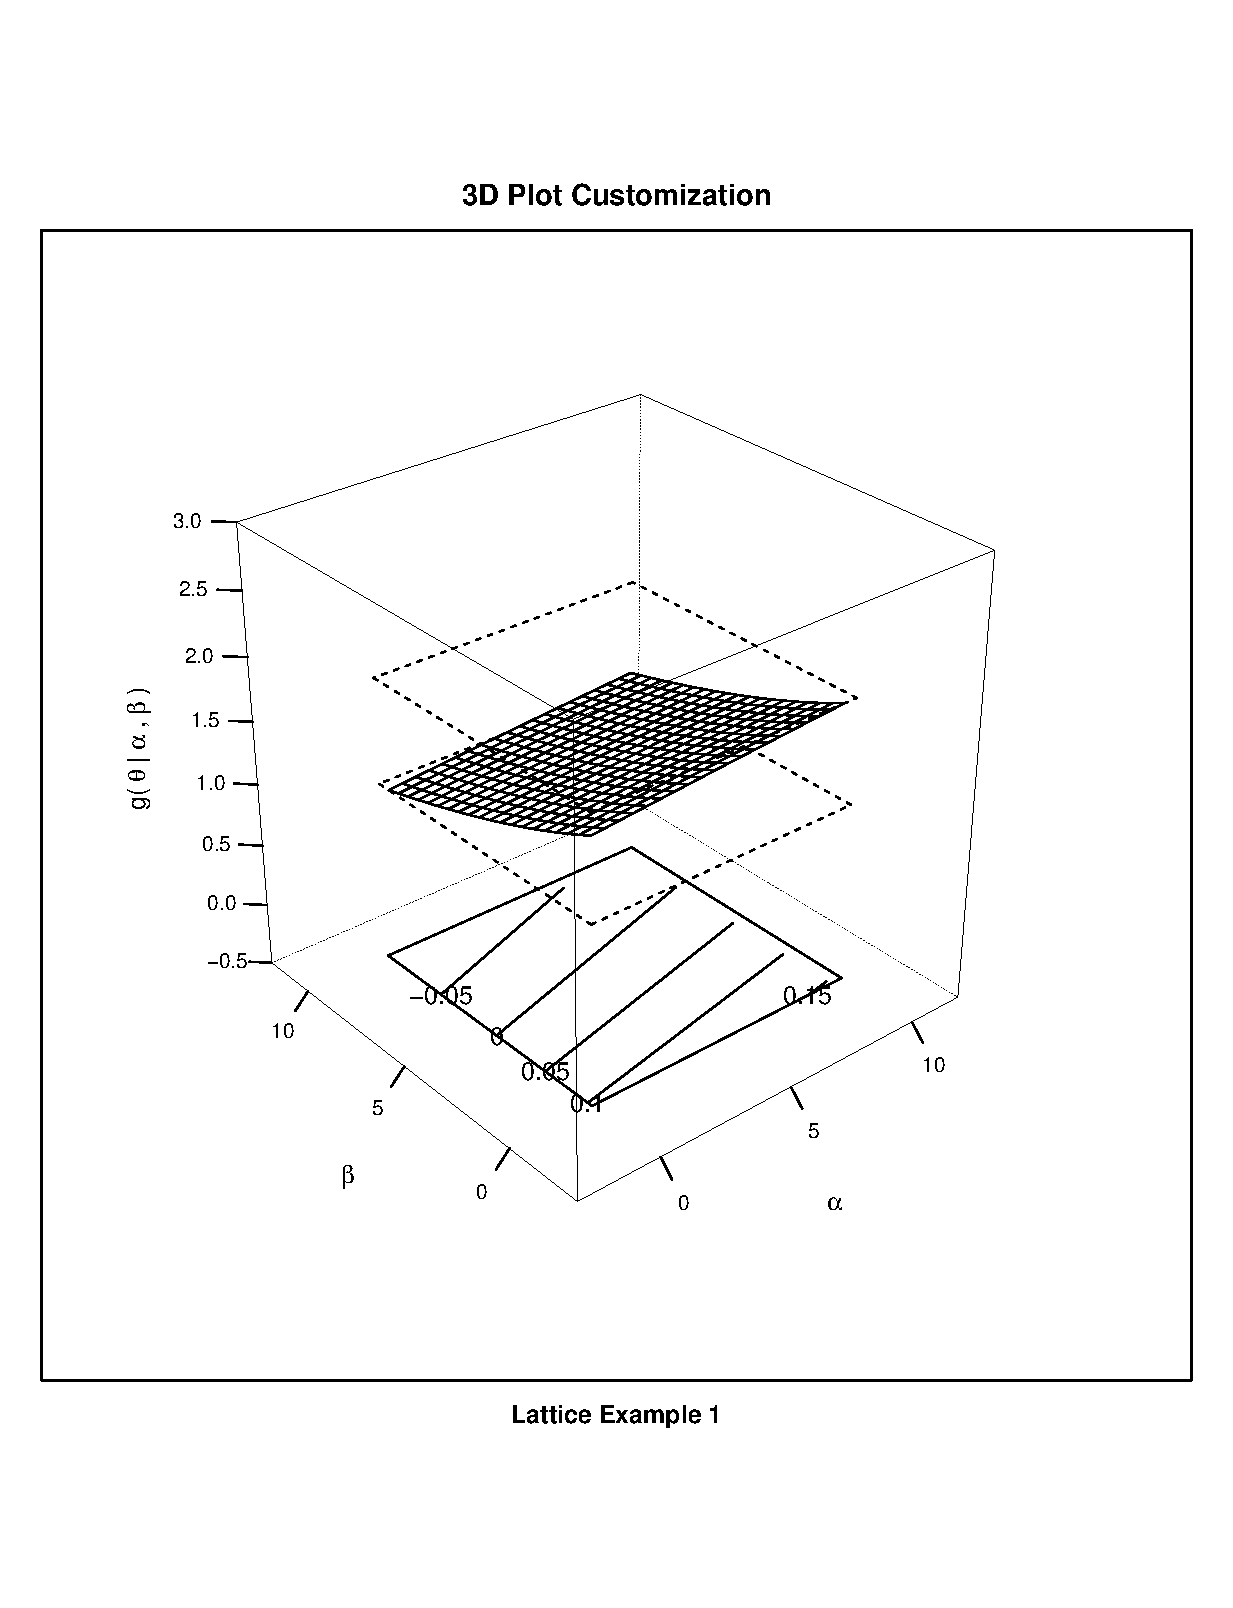
\includegraphics{./img/lattice-fig.eps}


\item \LaTeX 의 문서에 포함될 \texttt{.eps} 그래픽을 \texttt{R}에서 뽑았을 때는 아무런 문제가 없어 보였는데, 정작 \texttt{pdf}로 문서를 뽑아 보니까 이 그래픽이 들어간 페이지가 90도로 돌아가 있거나 혹은 그래픽이 90도로 회전되어 있을 경우에는 아래와 같이 하면 됩니다.

\begin{Schunk}
 \begin{Sinput}
  postscript(file=``filename.eps'', onefile=FALSE, horizontal=FALSE)
 \end{Sinput}
\end{Schunk}

이 문제에 대한 출처는 \texttt{postscript} 도움말입니다.

이문제를 다른 방법으로도 해결할 수 있습니다.  (대충 서너개 더 있음).

\item 새로운 그래픽 객체를 생성하는 방법을 설명해줘서 사용자가 추후에 독립적인 그래픽을 생성할 수 있게 도와주기 

	\item (접수: 2013-APR-23)  저는 다각형을 그리고 싶습니다. 
	
	\textsf{(답변)}  이것은 간단히 2차원-랜덤포인트 생성한 뒤에 \texttt{polygon()} 함수를 써서 보여주면 됨. 

\end{enumerate}

% ggplot2에서 stat_density2d에 오류가 있는것 같습니다. 모든 경우에 NA가 return된다는 보고











